\documentclass[%handout,
	sans,
	12pt,
	%slidescentered,% center text on slide
	%draft,			% compile as draft version
	%notes,			% include nodes in slides
	%compress		% compress navigation bar
]{beamer}

\beamertemplatenavigationsymbolsempty

\usetheme{default}
\usecolortheme{orchid}
\setbeamertemplate{frametitle}
{
    \vspace*{1.5em}\insertframetitle\vspace*{-1.5em}
}
\setbeamertemplate{footline}[frame number]

\usepackage[T1]{fontenc}
\usepackage[utf8x]{inputenc}

\usepackage{mathpazo}
\usepackage[british]{babel}
\usepackage{csquotes}

\newcommand{\high}[1]{{\usebeamercolor[fg]{structure} #1}}
\newcommand{\bad}[1]{\textcolor{red}{#1}}
\newcommand{\gray}[1]{\textcolor{darkgray}{#1}}
\newcommand{\black}[1]{\textcolor{black}{#1}}

\usepackage{amsmath,amssymb}
\usepackage{upgreek}
\usepackage{booktabs}
\usepackage{hyperref}
\usepackage{graphicx}
\usepackage{colortbl}
\usepackage{url}
\usepackage{setspace}
\usepackage{wrapfig}
\usepackage{tabularx}
\usepackage{xspace}
\usepackage{mathpartir}

\usepackage{tikz}
\usetikzlibrary{trees, positioning}
\usetikzlibrary{shapes.geometric}


\newcommand{\NN}{\mathbb{N}}
\newcommand{\QQ}{\mathbb{Q}}
\newcommand{\RR}{\mathbb{R}}
\newcommand{\CC}{\mathbb{C}}
\renewcommand{\epsilon}{\varepsilon}
\renewcommand{\phi}{\varphi}
\def\braces#1{[#1]}
\newcommand{\wrt}{w.\,r.\,t.\xspace}
\newcommand{\eg}{e.\,g.\xspace}
\newcommand{\ie}{i.\,e.\xspace}
\DeclareMathOperator\caret{\char`\^}

\newcommand{\hastype}{\,:\,}
\newcommand{\cons}{::}
\newcommand{\corrto}{\overset{\scriptscriptstyle\wedge}{=}}
\newcommand{\listapp}{\mathbin{@}}
\newcommand{\listnil}{[\hskip0.3mm]}
\newcommand{\listnth}{\mathbin{!}}
\newcommand{\expectation}{\text{\upshape E}}

\usepackage{manfnt}
\newenvironment{danger}{\medbreak\noindent\hangindent=2pc\hangafter=-2%
  \clubpenalty=10000%
  \hbox to0pt{\hskip-\hangindent\hskip0.25em\raisebox{-0.25em}[0pt][0pt]{\dbend}\hfill}\small\ignorespaces}%
  {\medbreak\par}
  %\raisebox{-1.05em}[0pt][0pt]{\Huge\hskip.15em \stixdanger}

\newcommand{\etAl}{\textit{et al.}\xspace}

%\definecolor{mybg}{rgb}{0.9,0.9,0.9}
\definecolor{mybg}{rgb}{1,1,1}
\setbeamercolor{background canvas}{bg=mybg}

\title{Field Extensions in \emph{Isabelle/HOL} \vspace*{-0.5em}}
\author{\normalsize Fabian Hellauer}
\institute[]{\footnotesize Technische Universität München}
\date{\footnotesize30 January 2019}

\begin{document}

\maketitle

\begin{frame}
\begin{center}
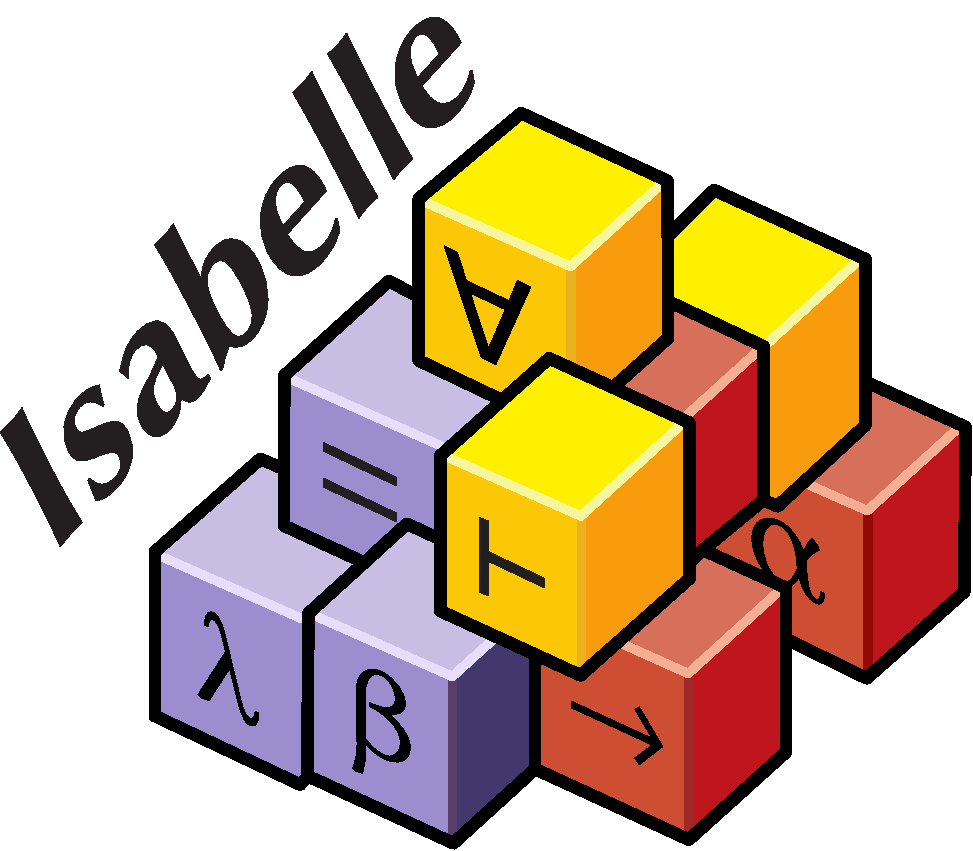
\includegraphics[width=5cm]{isabelle.pdf}
\end{center}
\end{frame}

\tableofcontents

\newcommand{\pivot}[1]{{\color{red}#1}}
\newcommand{\ltpiv}[1]{{\color{blue}#1}}
\newcommand{\gtpiv}[1]{{\color{olive}#1}}

\section{Verification of Mathematics}
\begin{frame}{Verification of Mathematics}%in particular widely accepted Mathematics like Linear Algebra
Reasons:
\begin{itemize}
	\item to obtain a basis for more useful results\pause
	%as a computer scientist, I mainly think of algorithms and their correctness
	\item to find mistakes\pause
	\item meta: to prove that verification %of a handfull of pages
	is feasible (when using modern tools)
	%this could be motivation to do more math theories, because it removes the need for experts to get them accepted.
\end{itemize}
\end{frame}

\section{Tool assistance}
\begin{frame}{Tool assistance}% how Isabelle helps in verifying
Isabelle enforces great precision, but also helps:
\begin{itemize}
	\item automatic proofs for simple lemmas\pause %rather: for *trivial* statements
	\item information about previously defined objects: \pause
	\includegraphics[width=0.7\linewidth]{"type_error"} \pause
	%also with control+click
	\item information about the proof state, e.g.\ pending sub-proofs
	%at any point in a proof. (example: induction over natural numbers).
	%And once again, simple sub-goals can be solved automatically.
\end{itemize}
\end{frame}

\section{HOL-Algebra}
\begin{frame}
\begin{center}
\huge\high{Algebraic Structures in HOL-Algebra}%Isabelle's library of abstract algebra, where groups and rings are defined
\end{center}
\end{frame}

\begin{frame}{HOL-Algebra}
\begin{itemize}
	\item record-based \pause%to-do: how to explain to Prof. K.?
	\item verbose (subscripts, ...) \pause%to-do: do they even appear in an example?
	\item locale-based \pause%INTEG as example?
	% reasons
	\item explicit carrier sets \pause
	\item enables reasoning about substructures	%this is what we will do
	% HOL-Computational_Algebra uses types --> this is not possible
\end{itemize}
\end{frame}

\subsection{Motivational Example}
\begin{frame}{Motivational Example}
	Why use HOL-Algebra?\pause
	
	\high{To formalise Galois theory!}\pause
	\begin{theorem}
		\upshape
		The polynomial $x^5 − x − 1$ has no root described by an expression of integers, $n$th roots and basic arithmetic operations.
	\end{theorem}\pause
	\bad{I won't get that far!}
\end{frame}

\section{Problems}
\begin{frame}{Problems}
\begin{itemize}
\item Bases are sets.
\bad{In the finite case, we often want them as lists. to-do: later? explain non-canonical}
\item Coefficients are functions.
\bad{need to prove membership in the correct function set at \emph{every} step.
	% at least that's what it feels like
	 to-do: details /example?}
\end{itemize}
\end{frame}

\subsection{to-do}
\begin{frame}{Encoding of $\infty$}%relevant?
Can we use type \emph{nat} for the degree of field extensions?\pause
\begin{itemize}
	\item The degree is a vector space dimension.\pause%these *can* be zero (iff zvs)
	\item However, it is always $\ge 1$.\pause
	\item Thus, this encoding strips no information:\\%It could be adapted easily to use extended natural numbers
	\textbf{definition} \textit{degree} \textbf{where}\\
	\hskip1em\textit{degree = (if finite then vs.dim else 0)}
\end{itemize}
\end{frame}

\section{Results} % what I contributed

\subsection{An explicit description of simple extensions}
\begin{frame}{An explicit description of simple extensions} %at least *more* explicit, still using set comprehension
%to-do: really interesting?
\end{frame}

\subsection{Classification of simple algebraic extensions}
\subsubsection{Minimal Polynomial}
\begin{frame}{Minimal Polynomial}%We are in a context where we have fixed L/K and some α∈L
\textbf{definition} \textit{irr} \textbf{where}\\
\hskip1em\textit{irr = (ARG-MIN degree p. p ∈ carrier P ∧ monic p ∧ Eval p = $\textbf{0}_L$)}\pause
\\[4mm]
\textbf{context}\\
\hskip1em\textbf{assumes} \textit{algebraic}\\
\textbf{begin}\\[2mm]\pause

(...38 lines later)\\[2mm]
\textbf{lemma} \textit{irr ∈ carrier P} \textbf{and} \textit{monic irr} \textbf{and} \textit{Eval irr = $\textbf{0}_L$}\\\pause
\textbf{and} \textit{irr ≠ \textbf{0}}\\\pause
\textbf{and} \textit{degree irr > 0}\pause
\\[3mm]
Uniqueness of the minimal polynomial takes another 180 lines. %But this is part of an actual proof, so this to be expected
%We keep that "algebraic" assumption for a bit...
\end{frame}

\subsection{Tower rule}
\begin{frame}{Tower rule}
If $M/L$ and $L/K$ are field extensions, then
\[[M : K] = [M : L] \cdot [L : K]\]\pause %ask M.: good idea to use non-HOL notation?
In particular, combining two finite field extensions yields a finite field extension. %(or combining finitely many)
\end{frame}

\subsection{Vector Spaces}
\begin{frame}{Vector Spaces}\pause
A \emph{vector space} $V$ over a field $K$ is an Abelian group (like $(\RR\times\RR,+,(0,0)$) together with a \emph{scale} operator $\odot:K\times V \to V$ which follows some (well-known) axioms.\pause
\begin{itemize}
\item $\RR \times \RR$ is a vector space over $\RR$.\pause
%these are coordinates in a 2d plane, we could also take 3d space
\item If $K$ is a field, then $\{0\}$ is a vector space over $K$.\pause
\item If $L/K$ is a field extension, then $L$ is a vector space over $K$.
\end{itemize}
\end{frame}

\subsection{Vector Spaces}
\begin{frame}{Results}
	\begin{theorem}
		If $n := dim(V) < \infty$, then $V \cong K^n$.
	\end{theorem}
\end{frame}
subspace-dim %needed base extension theorem

%to-do: more about nspace-iso problems?

\section{Contributions}
\begin{frame}{Contributions}
\begin{itemize}
	\item Vector Spaces: 850 lines, 75 lines preliminaries\pause
	\item Field Extensions: 820 lines, 100 lines preliminaries\pause%hard to distinguish
	\item 400 lines in an old development %annoying, mostly about subrings, which were not even defined when I started
	\item 120 lines example instantiations %to test definitions
	\item to-do: Maintenance work in the "VectorSpace" library
	\item Documentation: 300 lines (= 10 pages)
	%everything counted once
\end{itemize}
\end{frame}

\section{Field Extensions}
\begin{frame}
\begin{center}
\huge\high{Field Extensions}
\end{center}
\end{frame}

\begin{frame}
A \emph{field} is a nontrivial commutative ring where every nonzero element has a multiplicative inverse.
\pause %in addition to its additive inverse

A \emph{field extension} $L/K$ is a field $(\mkern-3mu\mid\mkern-6mu L,\otimes,1,\oplus,0\mkern-6mu\mid\mkern-3mu)$ where $K$ is a subset of $L$ and $(\mkern-3mu\mid\mkern-6mu K,\otimes,1,\oplus,0\mkern-6mu\mid\mkern-3mu)$ is again a field.
\begin{itemize}
\item If $K$ is a field, then $K/K$ is a field extension.\pause
%problem for a formalisation: K is often identified with its carrier set
\item $\RR/\QQ$ is a field extension.\pause
\item $\QQ(\sqrt{3})/\QQ$ is a field extension.
\end{itemize}
\end{frame}

\section{Conclusion}
\begin{frame}{Conclusion}
%to-do: partly stolen from Manuel
\begin{itemize}
\item Formalisation of textbook algebra is feasible with Isabelle.\pause
\item Some proofs get ugly due to a variety of reasons.\pause
\item Good libraries can help a lot.\pause\\[6mm] %to-do: as seen with the last result
%(If you don't like what you do, defer it to someone else)
\end{itemize}
Interesting project for HOL-Algebra:\\[2mm]
GaloisCVC by P.\ E.\ de Vilhena, M.\ Baillon and L.\ Paulson (ALEXANDRIA grant)
%so, I will keep an eye out on what happens to HOL-Algebra.
%If someone with push access wants to include my material, they can send me questions, I will try and answer them.
%The documentation is almost finished.
%Are there questions now?
\end{frame}

\section{Reference}
\begin{frame}{Reference}
	G.\ Kemper. Algebra. German lecture notes, 2018. \url{http://www-m11.ma.tum.de/fileadmin/w00bnb/www/people/kemper/lectureNotes/algebra\_nodates.pdf} 
\end{frame}

\end{document}
